
\section{Reguliere algoritmes}

\subsection{Inleiding}
Voordat we onderzoek kunnen doen naar zelflerende algoritmes moeten we eerst een beeld krijgen van reguliere algoritmes. Daarom behandelen we in dit hoofdstuk de vraag: \textit{Wat zijn voorbeelden van reguliere algoritmes en hoe werken ze?}


\subsection{Verschillende algoritmes}
Computers hebben geen bewustzijn. Om deze reden kunnen ze niet zelf bepalen iets te doen. Waar computers wel in uitblinken, is het uitvoeren van taken die hen zijn opgelegd. Vaak komen deze taken in de vorm van code. Via code kan je computers opdrachten geven, bijvoorbeeld: \textit{Bereken 7 * 6}. De boodschap valt echter niet op deze manier over te brengen. Afhankelijk van de taal waarin je programmeert zijn er vaste commando's waar de computer op zal reageren.
Naarmate de opdracht die je een computer wil laten uitvoeren complexer wordt, zal ook het gebruik van deze commando's ingewikkelder worden. Hier komen algoritmes in het spel. Een algoritme is een soort stappenplan, waarin een complexere handeling in duidelijke opdrachten weergegeven wordt. De volgende definitie geeft een betekenis in de meest algemene zin: \textit{"een algoritme is een eindige reeks instructies om vanaf een beginpunt een bepaald doel te bereiken."} \cite{WoordenOrg}

Een toegankelijke vergelijking is koken. Er is een \textbf{input} van voedsel waar uiteindelijk een gerecht uit moet komen, de \textbf{output}. Voor het tot stand komen van dit gerecht gebruik je misschien een recept. Dit recept is als het ware het algoritme.
Uit de gegeven definitie is af te leiden dat het aantal mogelijke algoritmes ontzettend groot is. Niet alleen is het een ruim begrip, ook kan het desbetreffende doel waarschijnlijk op meerdere manieren bereikt worden. Het ene algoritme zal misschien beter zijn dan het andere doordat het bijvoorbeeld effici\"enter werkt.

Uiteraard zijn er ook vele algoritmes die gebruik maken van toepassingen, zoals een \textbf{queue} en een \textbf{stack}, die betrekking hebben tot ons onderwerp. Enkele hiervan zullen hier beschreven worden.

\subsubsection{Breadth-first search (BFS)}
Dit algoritme, bedacht in de jaren vijftig van de vorige eeuw door E.F. Moore \cite{Moore}, een Amerikaans professor in de wiskunde en computer sciences en een voortrekker in kunstmatig leven, is een zoekalgoritme voor datasets in de vorm van grafieken of "boom"-structuren. In deze dataset wordt een \textbf{node} als oorsprong benoemd, de \textbf{root}. Ook wordt een bepaalde uitkomst als doel gesteld. Vervolgens krijgt elke node drie waardes aangewezen:
\begin{itemize}
\item De afstand van de huidige node naar de root. Dit is het aantal stappen dat gezet moet worden om bij de root te komen. 
\item De node die v\'{o}\'{o}r de huidige node kwam, de \textbf{predecessor}. Anders gezegd: bij welke node je uitkomt als je een enkele stap terug zet.
\item Een \textbf{state}. De state houdt bij of de node al gecontroleerd is.
\end{itemize}

Bij Breadth-first search wordt gebruik gemaakt van een queue. Dit is een lijst waar nodes aan toegevoegd en uitgehaald kunnen worden. Net zoals een daadwerkelijke wachtrij wordt het "\textit{eerste erin, als eerste eruit}" principe toegepast.
Het Breadth-first search algoritme ziet er als volgt uit:

\begin{enumerate}
\item Maak een lege lijst S voor bezochte nodes.
\item Maak een lege lijst Q met de queue.
\item Benoem \'e\'en node als root en voeg deze toe aan S.
\item Voeg de root toe aan Q. 
\item Zolang Q niet leeg is:
	\begin{enumerate}
	\item Haal de voorste node uit de queue. Dit is de \textit{current} node.
	\item Als current het doel is:
		\begin{enumerate}
		\item Return current.
		\end{enumerate}
	\item Voor elke node die grenst* aan current:
		\begin{enumerate}
		\item Als deze node nog niet bezocht is en dus niet in S zit:
			\begin{enumerate}
			\item Voeg de node toe aan S.
			\item Zeg dat de predecessor van de node de current node is.
			\item Haal de node uit de queue.
			\end{enumerate}
		\end{enumerate}
	\end{enumerate}
\end{enumerate}

\textit{*Aangrenzend zijn betekent hier \textit{in directe verbinding staan met}.}

\begin{figure}[h]
  \centering
    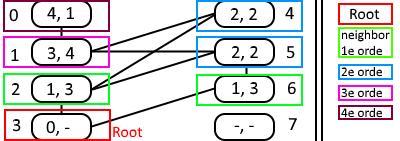
\includegraphics[width=\textwidth]{datasetBFS3.png}
  \caption{Schematische weergave van een willekeurige dataset. Waarop het Breadth-first search algoritme wordt toegepast.}
  \label{fig:datasetBFS3}
\end{figure}
Hierboven is een voorbeeld van een simpele dataset weergegeven (zie figuur \ref{fig:datasetBFS3}), genummerd van node 0 tot en met node 6. Node 3 is de root en node 0 het doel. Om bij het doel te komen wordt het Breadth-first search algoritme toegepast. Node 3, de root, wordt toegevoegd aan de lijsten Q en S. Node 3 wordt weer uit de queue gehaald en \'e\'en voor \'e\'en worden de aangrenzende nodes bekeken. Hierbij worden ze toegevoegd aan de stack. Omdat zowel 2 als 6 het niet het doel zijn, herhaald het algoritme zich. Nu wordt 2 bekeken. Het doel is niet gevonden in de aangrenzende nodes. Daarna komt 6, ook zonder succes. (Let hierbij op dat node 5 niet nogmaals bekeken wordt, dit is namelijk als bij node 2 gedaan en is dus al aanwezig in lijst S). Intussen zijn node 4 en node 5 toegevoegd aan de queue, ze zijn immers verbonden met node 2. Ook hier wordt het proces herhaald, node 1 zit nu in de queue. Uiteindelijk wordt node 1 bekeken en wordt het doel, node 0, gevonden.

Met BFS kan je zo de weg van de root naar het doel achterhalen. Dit is nuttig als je bijvoorbeeld een wegennetwerk hebt en wil weten wat de kortste weg van de ene naar de andere stad is.


\subsubsection{Depth-first search (DFS)}
Evenals breadth-first search is depth-first search een algoritme voor het doorlopen van datasets in de vorm van grafieken of trees. DFS verschilt echter op twee manieren van BFS:

\begin{itemize}
\item Depth-first search gebruikt een stack in plaats van een queue. Waar nodes in een BFS systeem in een wachtrij werden geplaats met een "als eerst erin, als eerst eruit" principe, handhaaft een DFS systeem een wachtrij meer vergelijkbaar met een stapel papieren. Telkens pak je het bovenste element van de stapel om mee te werken, maar als je iets in de wachtrij stopt, komt dit ook weer bovenop de stapel te liggen. De meest recente toevoeging zal dus als eerste weer eruit gehaald worden.
\item Breadth-first search begon bij een root. Vervolgens werd gekeken naar alle neighbors. Als de gewenste uitkomst niet tussen deze neighbors zit, worden de neighbors van deze neighbors gecontroleerd. Dit proces herhaalt zich totdat het doel gevonden is.
Depth-first search begint ook bij een root, maar kijkt direct naar een weg tot een node bereikt is die geen neighbors meer heeft. Als het doel dan niet bereikt is wordt een andere weg geprobeerd. Hiervoor wordt gebruik gemaakt van \textbf{recursive backtracking}.

\end{itemize}

\begin{figure}[H]
  \centering
    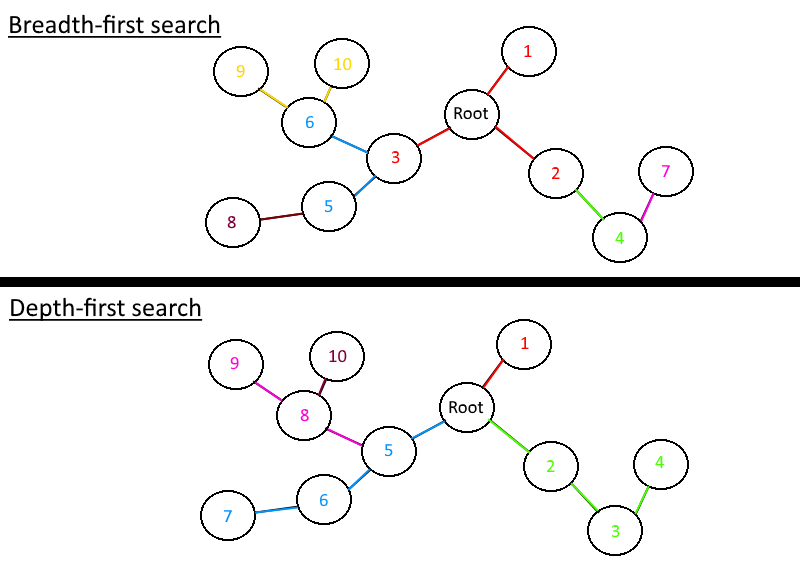
\includegraphics[width=\textwidth]{verschil-BFS-DFS.png}
  \caption{Schematische weergave van een willekeurige dataset.}
  \label{fig:verschil-BFS-DFS}
\end{figure}

In figuur \ref{fig:verschil-BFS-DFS} is de werking van BFS en DFS weergegeven. Het getal in elke node geeft aan als hoeveelste het bereikt wordt. 

Ook bij DFS hebben de nodes een state: bezocht of niet bezocht.
Ten eerste wordt de root gekozen en deze wordt als bezocht opgeslagen. Zoals te zien wordt er vanaf de root \'e\'en (willekeurige) neighbor gekozen om te onderzoeken. Elke bezochte neighbor wordt als bezocht genoteerd. De root wordt in de stack geplaats. Vanaf deze neighbor wordt weer een nieuwe aanliggende node gekozen, waarvan de state 'onbezocht' is. Nu ook wordt de bezochte node in de stack geplaatst. Dit proces herhaalt zich totdat er een node is zonder (onbezochte) neighbors. Op dat moment wordt de bovenste node uit de stack gehaald, dit heet backtracking, en herhaalt het proces zich. Dit blijft doorgaan totdat geen enkele node onbezochte neighbors over heeft of totdat het doel gevonden is.

Als vuistregel kan het volgende gehanteerd worden: depth-first search wordt gebruikt als je weet dat er maar \'e\'en uitkomst is, breadth-first search als je de makkelijkste of snelste uitkomst wil kiezen.

\subsection{Conclusie}
Twee voorbeelden van reguliere algoritmes zijn "Breadth-first seach" en  "Depth-first search". Dit zijn twee algoritmes met vele toepassingen. Beide algoritmes zijn niet zelflerend omdat ze hun manier van zoeken niet zelf verbeteren.
\newpage

\textcolor{praktijk}{
\subsection{Praktijk: Voorbeelden algoritmes}
}

Algoritmes hebben meestal vele toepassingen. Hier zijn enkele voorbeelden van de eerder genoemde algoritmes.
\subsubsection{Breadth-first search}
\begin{figure}[h]
  \centering
    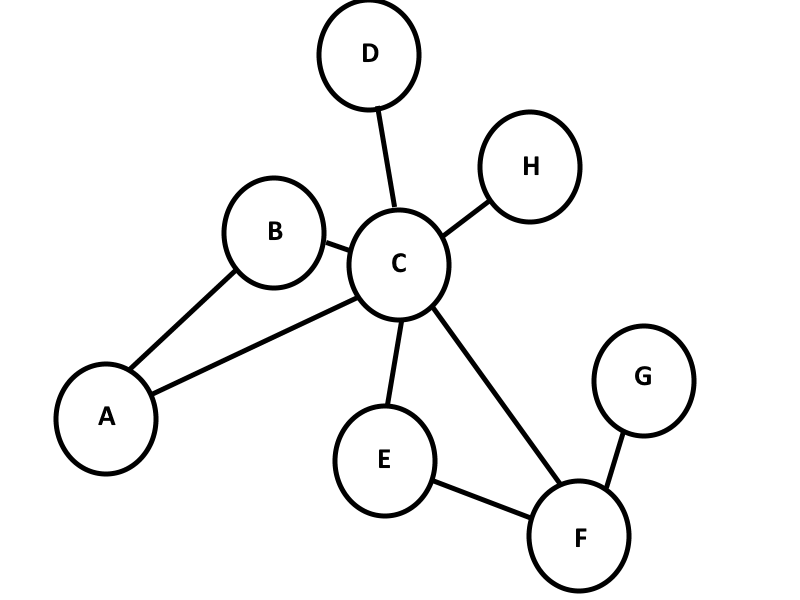
\includegraphics[width=0.8\textwidth]{datasetBFS2.png}
  \caption{Schematische weergave van een willekeurige dataset.}
  \label{fig:datasetBFS2}
\end{figure}

In figuur \ref{fig:datasetBFS2} is een dataset te zien, bijvoorbeeld een telefoonboom. Elke cirkel representeert een persoon. Zo kan persoon A de personen B en C bellen, maar A bezit geen andere telefoonnummers. Toch zou hij een boodschap naar H kunnen sturen: via C. 
Stel, persoon A wil nu iets tegen F zeggen. In een kleine dataset als deze is makkelijk met het oog te zien dat de snelste manier hiervoor A – C – F is en dat A – B – C – E – F veel langer is. Bij grotere datasets is dit echter al snel moeilijk met zekerheid te zeggen. Hiervoor kan breadth-first search ingezet worden.

\subsubsection{Depth-first search}

\begin{figure}[H]
  \centering
    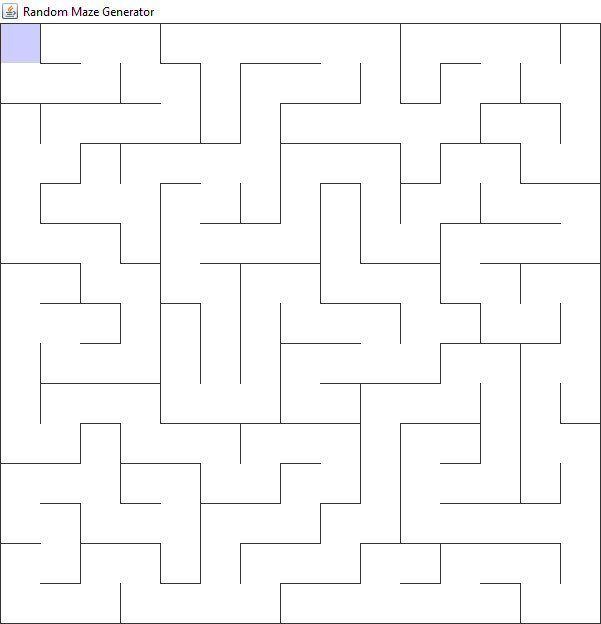
\includegraphics[width=0.8\textwidth]{maze.png}
  \caption{Een voorbeeld van een automatisch gegenereerd doolhof, gebruik makend van DFS.}
  \label{fig:maze}
\end{figure}

Depth-first search kan gebruikt worden voor zowel het maken als oplossen van doolhoven. In figuur \ref{fig:maze} is een doolhof te zien dat gemaakt is met behulp van DFS. Wij hebben in het kader van deze deelvraag een doolhof-generator gemaakt. Het algoritme in de vorm van een stappenplan is als volgt:

\begin{enumerate}
\item Maak de start cel current en markeer deze als bezocht.
\item Terwijl er nog niet bezochte cellen aanwezig zijn:
	\begin{enumerate}
	\item Als current neighbors heeft die nog niet bezocht zijn:
		\begin{enumerate}
		\item Kies willekeurig een van de neighbors
		\item Voeg current toe aan de stack
		\item Verwijder de muur tussen de huidige cel en de gekozen cel
		\item Benoem de gekozen cel als current en zet de state op bezocht
		\item Kies willekeurig een van de neighbors.
		\item Voeg current toe aan de stack.
		\item Verwijder de muur tussen de huidige cel en de gekozen cel.
		\item Benoem de gekozen cel als current en zet de state op bezocht.
		\end{enumerate}			
	
	\item Anders, als de stack niet leeg is:
		\begin{enumerate}
		\item Haal de laatst toegevoegde cel uit de stack en verwijder deze hieruit
		\item Maak deze cel current
		\item Haal de laatst toegevoegde cel uit de stack en verwijder deze hieruit.
		\item Maak deze cel current.
		\end{enumerate}	
	\end{enumerate}
\end{enumerate}
